\documentclass[margin=5mm]{standalone}
\usepackage[dvipsnames]{xcolor}
\usepackage{pgfplots}
\usepackage{tikz}
\usepackage[tikz]{ocgx2}

\pgfplotsset{compat=1.18}
\begin{document}

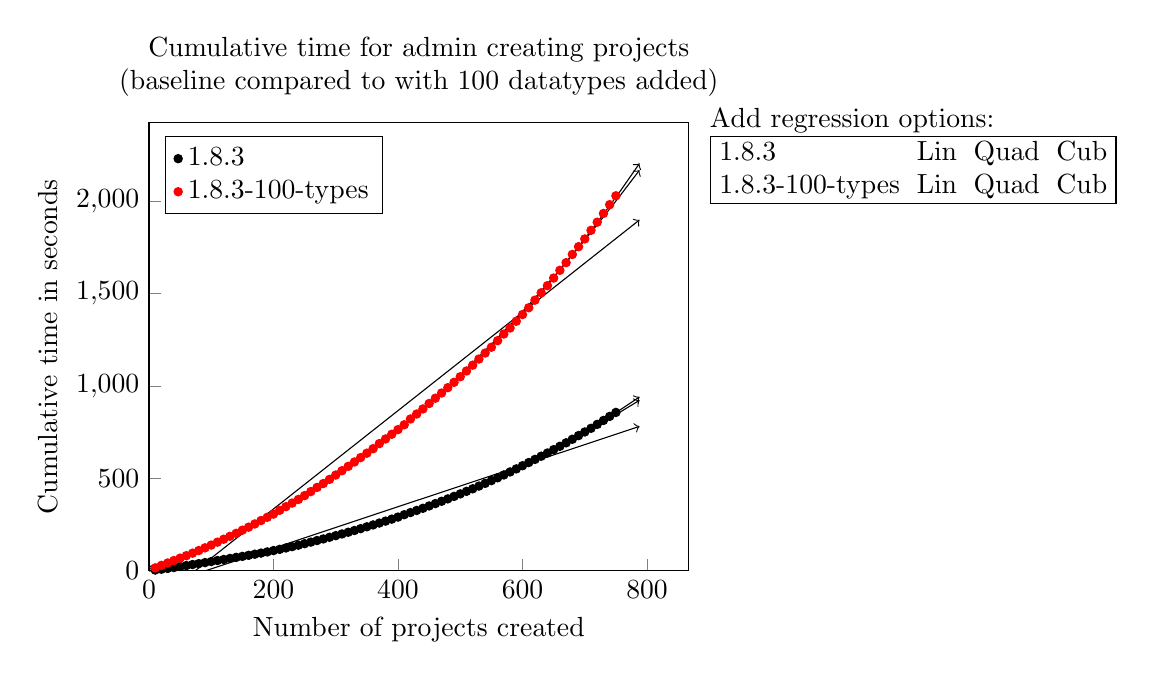
\begin{tikzpicture}
    \begin{axis}[
        align = center,
        legend pos = north west,
        legend cell align = left,
        xlabel = Number of projects created,
        ylabel = Cumulative time in seconds,
        xtick pos = left,
        ytick pos = left,
        scaled ticks = false,
        xmin = 0,
        ymin = 0,
        title = {Cumulative time for admin creating projects (baseline compared to with 100 datatypes added)},
        title style = {text width = 0.8\textwidth},
        legend entries={\switchocg{1.8.3}{1.8.3},\switchocg{1.8.3-100-types}{1.8.3-100-types}}]
        \begin{scope}[ocg = {ref = 1.8.3-Lin, status = invisible}]
            \plot[domain=0:788,->,forget plot] (\x,{-100.8889578378377365197593462653458118438720703125 + 1.1205677837837837440559951573959551751613616943359375*(\x)^1});
        \end{scope}
        \begin{scope}[ocg = {ref = 1.8.3-Quad, status = invisible}]
            \plot[domain=0:788,->,forget plot] (\x,{14.23812250277669733122820616699755191802978515625 + 0.2234736512595147106541304538041003979742527008056640625*(\x)^1 + 0.00118038701647930183678825155624281251220963895320892333984375*(\x)^2});
        \end{scope}
        \begin{scope}[ocg = {ref = 1.8.3-Cub, status = invisible}]
            \plot[domain=0:788,->,forget plot] (\x,{1.80406539141892086064444811199791729450225830078125 + 0.413535570211979230936805151941371150314807891845703125*(\x)^1 + 0.000559305242685200995102212662146712318644858896732330322265625*(\x)^2 + 0.0000005448085735035974346202915230552576986156054772436618804931640625*(\x)^3});
        \end{scope}
        \begin{scope}[ocg = {ref = 1.8.3, status = visible}]
            \addplot[
                only marks,
                color = black,
                mark = *,
                mark size = 1.5 pt
            ]coordinates {(10,4.886)(20,9.387)(30,13.681)(40,18.501)(50,24.062)(60,29.147)(70,34.597)(80,39.645)(90,45.154)(100,50.897)(110,56.434)(120,61.942)(130,67.637)(140,73.313)(150,78.749)(160,84.578)(170,90.495)(180,96.631)(190,102.942)(200,110.163)(210,116.903)(220,124.226)(230,131.514)(240,139.348)(250,147.297)(260,155.97)(270,164.601)(280,173.214)(290,182.067)(300,190.904)(310,200.112)(320,209.237)(330,218.906)(340,228.921)(350,238.836)(360,248.867)(370,259.117)(380,269.49)(390,280.207)(400,291.467)(410,304.205)(420,315.733)(430,327.268)(440,338.969)(450,351.543)(460,364.253)(470,376.89)(480,389.826)(490,403.253)(500,416.864)(510,430.664)(520,444.528)(530,459.098)(540,473.74)(550,488.85)(560,503.928)(570,519.235)(580,535.549)(590,552.117)(600,569.137)(610,586.296)(620,603.279)(630,620.603)(640,637.999)(650,655.999)(660,674.161)(670,693.038)(680,712.355)(690,732.1)(700,751.812)(710,771.631)(720,792.924)(730,814.127)(740,836.013)(750,857.478)};
        \end{scope}
        \begin{scope}[ocg = {ref = 1.8.3-100-types-Lin, status = invisible}]
            \plot[domain=0:788,->,forget plot] (\x,{-196.5823207207207587998709641396999359130859375 + 2.659537510668563253801721657509915530681610107421875*(\x)^1});
        \end{scope}
        \begin{scope}[ocg = {ref = 1.8.3-100-types-Quad, status = invisible}]
            \plot[domain=0:788,->,forget plot] (\x,{22.942130988522546175545357982628047466278076171875 + 0.94895736747965420132544522857642732560634613037109375*(\x)^1 + 0.0022507633463011967288325276825844412087462842464447021484375*(\x)^2});
        \end{scope}
        \begin{scope}[ocg = {ref = 1.8.3-100-types-Cub, status = invisible}]
            \plot[domain=0:788,->,forget plot] (\x,{-1.8341494713893784496150374252465553581714630126953125 + 1.3276774719911454969434316808474250137805938720703125*(\x)^1 + 0.00101318689975214985994622640674833746743388473987579345703125*(\x)^2 + 0.00000108559337416583097756634344877024744846494286321103572845458984375*(\x)^3});
        \end{scope}
        \begin{scope}[ocg = {ref = 1.8.3-100-types, status = visible}]
            \addplot[
                only marks,
                color = red,
                mark = *,
                mark size = 1.5 pt
            ]coordinates {(10,16.558)(20,30.412)(30,42.997)(40,56.169)(50,69.296)(60,82.513)(70,96.229)(80,110.315)(90,125.042)(100,139.959)(110,155.81)(120,171.612)(130,187.391)(140,203.369)(150,220.582)(160,236.894)(170,254.203)(180,272.612)(190,290.284)(200,307.661)(210,328.003)(220,347.767)(230,367.122)(240,386.778)(250,407.547)(260,429.339)(270,451.846)(280,472.967)(290,495.274)(300,518.911)(310,542.218)(320,565.789)(330,589.391)(340,613.092)(350,637.072)(360,661.342)(370,688.862)(380,714.057)(390,739.417)(400,764.64)(410,790.658)(420,821.965)(430,848.947)(440,876.347)(450,905.648)(460,934.453)(470,962.449)(480,991.382)(490,1020.427)(500,1050.579)(510,1081.734)(520,1113.172)(530,1146.283)(540,1178.764)(550,1210.053)(560,1245.615)(570,1281.661)(580,1314.083)(590,1350.795)(600,1387.003)(610,1423.759)(620,1464.862)(630,1504.679)(640,1542.998)(650,1584.399)(660,1626.256)(670,1667.757)(680,1711.989)(690,1753.95)(700,1795.977)(710,1842.48)(720,1886.432)(730,1933.66)(740,1981.157)(750,2029.43)};
        \end{scope}
    \end{axis}
    \begin{scope}
        \addtolength{\tabcolsep}{-0.3em}
        \node [below right, shape=rectangle, align=left](regressiontable) at (7,6) {
            Add regression options: \\
            \begin{tabular}{|llll|}
                \hline
                1.8.3 & \switchocg{1.8.3-Lin}{Lin} & \switchocg{1.8.3-Quad}{Quad} & \switchocg{1.8.3-Cub}{Cub} \\
                1.8.3-100-types & \switchocg{1.8.3-100-types-Lin}{Lin} & \switchocg{1.8.3-100-types-Quad}{Quad} & \switchocg{1.8.3-100-types-Cub}{Cub} \\
                \hline
            \end{tabular}
        };
    \end{scope}
\end{tikzpicture}

\end{document}